\documentclass[xcolor=x11names,compress,10pt]{beamer}

\usepackage{booktabs}
\usepackage{graphicx}
\usepackage{epstopdf}
\epstopdfsetup{outdir=./}
\usepackage[english]{babel}
\usepackage[utf8]{inputenc}
\usepackage{tikz}
\usetikzlibrary{decorations.fractals}
\usepackage{amsmath}
\usepackage{amsfonts}

% \usepackage{caption}
\usepackage{algorithm}
\usepackage{algorithmic}
\floatname{algorithm}{Algoritmo}
\renewcommand{\listalgorithmname}{Lista de algoritmos}
\renewcommand{\algorithmicrequire}{\textbf{Entrada:}}
\renewcommand{\algorithmicensure}{\textbf{Salida:}}
\renewcommand{\algorithmicend}{\textbf{fin}}
\renewcommand{\algorithmicif}{\textbf{si}}
\renewcommand{\algorithmicthen}{\textbf{entonces}}
\renewcommand{\algorithmicelse}{\textbf{si no}}
\renewcommand{\algorithmicelsif}{\algorithmicelse,\ \algorithmicif}
\renewcommand{\algorithmicendif}{\algorithmicend\ \algorithmicif}
\renewcommand{\algorithmicfor}{\textbf{para}}
\renewcommand{\algorithmicforall}{\textbf{para todo}}
\renewcommand{\algorithmicdo}{\textbf{hacer}}
\renewcommand{\algorithmicendfor}{\algorithmicend\ \algorithmicfor}
\renewcommand{\algorithmicwhile}{\textbf{mientras}}
\renewcommand{\algorithmicendwhile}{\algorithmicend\ \algorithmicwhile}
\renewcommand{\algorithmicloop}{\textbf{repetir}}
\renewcommand{\algorithmicendloop}{\algorithmicend\ \algorithmicloop}
\renewcommand{\algorithmicrepeat}{\textbf{repetir}}
\renewcommand{\algorithmicuntil}{\textbf{hasta que}}
\renewcommand{\algorithmicprint}{\textbf{imprimir}} 
\renewcommand{\algorithmicreturn}{\textbf{devolver}} 
\renewcommand{\algorithmictrue}{\textbf{cierto }} 
\renewcommand{\algorithmicfalse}{\textbf{falso }} 

\useoutertheme[subsection=false,shadow]{miniframes}
\useinnertheme{default}
\usefonttheme{serif}
\usepackage{palatino}

\setbeamerfont{title like}{shape=\scshape}
\setbeamerfont{frametitle}{shape=\scshape}

\setbeamercolor*{lower separation line head}{bg=DeepSkyBlue4} 
\setbeamercolor*{normal text}{fg=black,bg=white} 
\setbeamercolor*{alerted text}{fg=red} 
\setbeamercolor*{example text}{fg=blue} 
\setbeamercolor*{structure}{fg=black} 
\setbeamercolor{block body}{bg=normal text.bg!90!black}
\setbeamercolor{block title}{fg=white,bg=normal text.bg!40!black}


\setbeamercolor*{palette tertiary}{fg=black,bg=black!10} 
\setbeamercolor*{palette quaternary}{fg=black,bg=black!10} 

\renewcommand{\(}{\begin{columns}}
\renewcommand{\)}{\end{columns}}
\newcommand{\<}[1]{\begin{column}{#1}}
\renewcommand{\>}{\end{column}}

\begin{document}

\begin{frame}
\title{\large{PCA, Principal Components Analysis}}
\subtitle{Fundamentals}
\author{
	{\scriptsize Rafael Pérez Torres\\
	Selected Topics on Pattern Recognition\\
	Profesor: Dr. Wilfrido Gómez Flores\\
	}{\it LTI Cinvestav}\\
}
\date{
	\begin{tikzpicture}[decoration=Koch curve type 2] 
		\draw[DeepSkyBlue4] decorate{ decorate{ decorate{ (0,0) -- (3,0) }}}; 
	\end{tikzpicture}  
	\\
	\vspace{0.2cm}
	Jun 19th, 2015
}
\titlepage
\end{frame}

\begin{frame}{Agenda}
\tableofcontents
\end{frame}


\section{\scshape Introduction}
\subsection{Introduction}
\begin{frame}{Why to reduce dimensionality?}
\begin{block}{The curse of dimensionality}
\begin{itemize}
	\item Coined by Bellman in 1961.
	\item The size of sample for estimating a multivariate function increases exponentially to the number of variables.
	\item \textbf{More variables, more computational cost.}
\end{itemize}
\end{block}

\end{frame}
\begin{frame}{Why to reduce dimensionality? II}
\begin{block}{Sparse space phenomenom}
\begin{itemize}
	\item Coined by Scott and Thompson.
	\item The actual guilty of \emph{the curse of dimensionality}.
	\item High-dimensional spaces are inherently sparse.
\end{itemize}
\end{block}
\begin{block}{Intrinsic dimension}
\begin{itemize}
	\item The precursor for looking at dimensionality reduction.
	\item It refers to the amount of independent variables enough for describing a phenomenom.
\end{itemize}
\end{block}
\end{frame}

\subsection{Dimensionality reduction}
\begin{frame}{Dimensionality reduction}
\begin{block}{Definition}
\begin{itemize}
	\item Given a set of features, select the most important ones for reducing the set's size, keeping the maximum discriminatory information as possible.
	\item Typically, many of the features are less representative than noise in data, becoming irrelevant.
	\item Typically, many of the features are correlated between themselves.
\end{itemize}
\end{block}
\end{frame}

\begin{frame}{Dimensionality reduction types}
\begin{block}{Types}
\begin{itemize}
	\item \textbf{Features' Extraction-Generation}: Given a features set $\mathbf{x}_i \in \mathbb{R} ^M$, find a mapping $\mathbf{y} = f(x):\mathbb{R}^M \to \mathbb{R}^m$, with $m<M$, such as the transformed vector $\mathbf{y}_i \in \mathbb{R}^m$ \textbf{\emph{preserves information}} in $\mathbb{R}^M$.
	\item \textbf{Features selection}: Given a features set $\mathbf{x}_i = \left \{ x_j | j = 1, \ldots, M  \right \}$ find a subset $\mathbf{y}_i=\left \{x_{i1},\ldots,x_{im} \right \}$, with $m<M$, such as it \textbf{\emph{maximizes the performance}} of classification.
\end{itemize}
\end{block}

\begin{columns}[onlytextwidth]
    \begin{column}{0.45\textwidth}
      \centering
      		$	
		\begin{bmatrix}
			x_1\\ 
			x_2\\ 
			\vdots\\ 
			x_M\\ 
			\end{bmatrix}
			\to
			\begin{bmatrix}
			y_1\\ 
			y_2\\ 
			\vdots\\ 
			y_M\\ 
			\end{bmatrix}
			=f \left (
			\begin{bmatrix}
			x_1\\ 
			x_2\\ 
			\vdots\\ 
			x_3\\ 
			\end{bmatrix}
			\right ) 
		$
		{\small Features extraction}
    \end{column}
    \begin{column}{0.45\textwidth}
      \centering
      $
	\begin{bmatrix}
	x_1\\ 
	x_2\\ 
	\vdots\\ 
	x_M\\ 
	\end{bmatrix}
	\to
	\begin{bmatrix}
	x_{i1}\\ 
	x_{i2}\\ 
	\vdots\\ 
	x_{iM}\\ 
	\end{bmatrix}
	$

	{\small Features selection}
    \end{column}
    \end{columns}
\end{frame}

\section{\scshape PCA Fundamentals}
\subsection{Fundamentals}
\begin{frame}{Principal Component Analysis PCA}
\begin{block}{Basic idea}
\begin{itemize}
	\item Tries to identify most significant basis (perspectives) for re-expressing a data set, filtering the noise and revealing hidden structures.
\end{itemize}

\begin{figure}
	\centering
	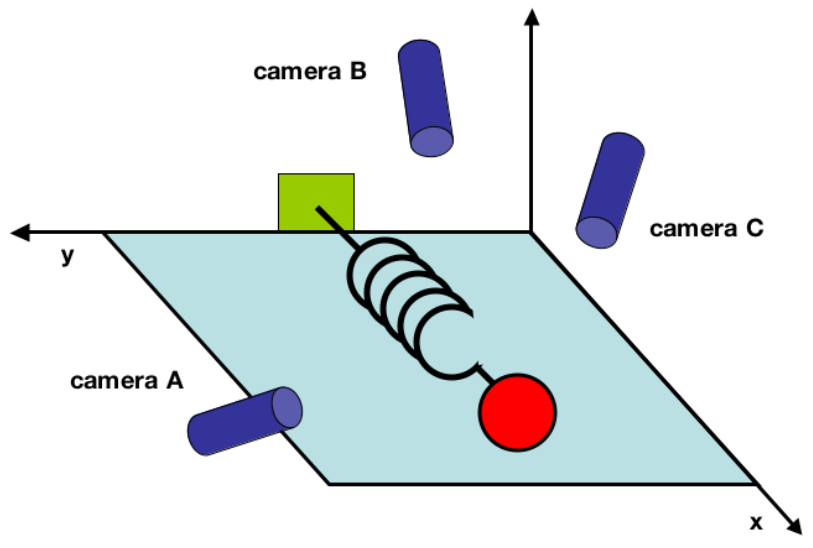
\includegraphics[scale=0.2]{../report/resources/images/resorte}
	\caption{Different perspectives of problem and associated features}
	\label{fig:figure1}
\end{figure}
\end{block}
\end{frame}

\begin{frame}{Principal Component Analysis PCA II}
\begin{block}{Basic idea}
\begin{itemize}
	\item We know $\overrightarrow{x}$ axis describes by itself the movement of the spring, but we don't know even what an axis is, we only have the raw perspectives given by data.
	\begin{figure}
	\centering
	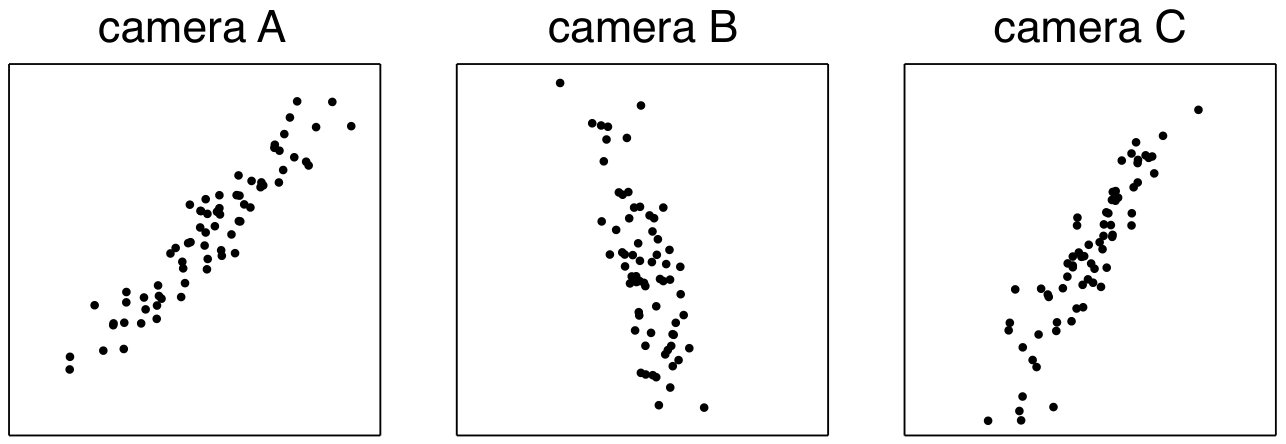
\includegraphics[scale=0.2]{../report/resources/images/camaras}
	\caption{Data read from real world}
	\label{fig:figure2}
\end{figure}
	\item How to migrate from perspectives in Figure to the successful $\overrightarrow{x}$ perspective?
\end{itemize}
\end{block}
\end{frame}


\begin{frame}{Principal Component Analysis PCA III}
\begin{block}{Basic idea}
\begin{itemize}
	\item Data can be expressed as a linear combination of its basis vectors.
	\item Let $\mathbf{X}$ a $m \times n$ matrix with the original data set, $\mathbf{Y}$ another $m \times n$ matrix for storing a new data representation built from matrix $\mathbf{P}$, such as $\mathbf{PX} = \mathbf{Y}$.
\end{itemize}
\begin{columns}[onlytextwidth]
    \begin{column}{0.45\textwidth}
      \centering
      		$
		\mathbf{PX} =
\begin{bmatrix}
p_1 \\ \vdots \\ p_m
\end{bmatrix}
\begin{bmatrix}
x_1 & \cdots & x_n
\end{bmatrix}
		$
    \end{column}
    \begin{column}{0.45\textwidth}
      \centering
      $
	Y =
\begin{bmatrix}
p_1x_1 & \ldots & p_1x_n\\ 
\vdots & \ddots & \vdots \\ 
p_mx_1 & \cdots & p_mx_n
\\ 

\end{bmatrix}
	$
    \end{column}
    \end{columns}
    {\center \small New basis vectors}
\end{block}
\end{frame}

\begin{frame}{Principal Component Analysis PCA IV}
\begin{block}{Basic idea}
\begin{itemize}
	\item Geometrically, $P$ is a rotation and a stretch transforming $\mathbf{X}$ into $\mathbf{Y}$
	\item Rows of $\mathbf{P}$, $\left \{ p_1,\ldots,p_m \right \}$ are the new set of basis vectors for representing $\mathbf{X}$.
	\item The $j$-th coefficient of $y_i$ is a projectionover the  $j$-ith row of $\mathbf{P}$
\end{itemize}
\end{block}
\end{frame}

\subsection{Elementr for data description}
\begin{frame}{Elements for data description}
\begin{block}{Noise and rotation}
$$
SNR = \frac{\sigma^2_{\text{signal}}}{\sigma^2_{\text{noise}}}
$$
\begin{itemize}
	\item A high SNR value means high accuracy, a low value indicates noise.
	\begin{figure}
	\centering
	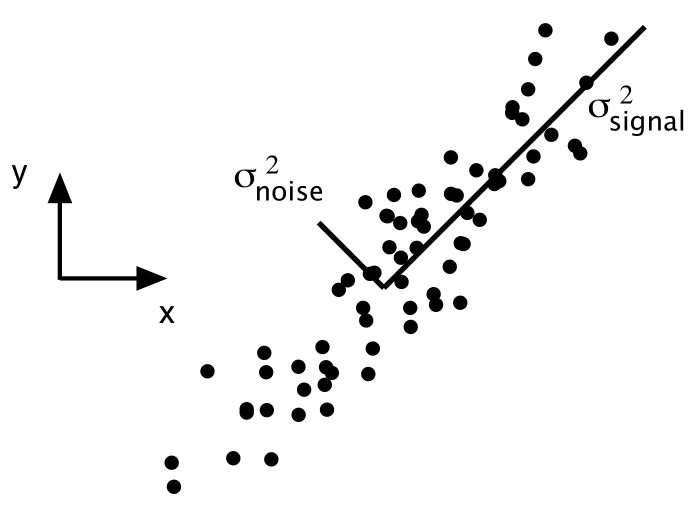
\includegraphics[scale=0.2]{../report/resources/images/snr}
	\caption{SNR and variance relation}
	\label{fig:snr-variance}
\end{figure}
\end{itemize}
\end{block}
\end{frame}

\begin{frame}{Elements for data description II}
\begin{block}{Redundancy}
\begin{itemize}
	\item If you can explain attribute $r2$ from attribute $r1$, then they are correlated.
	\item The goal is to reduce the amount correlated variables.
	\begin{figure}
	\centering
	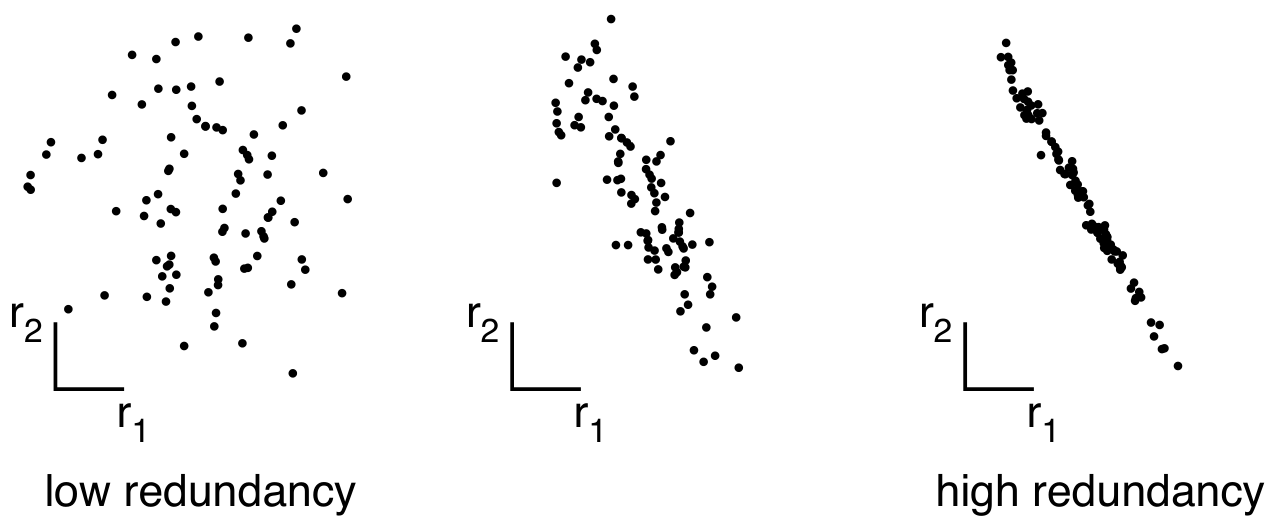
\includegraphics[scale=0.2]{../report/resources/images/redundancia}
	\caption{Different degrees of data redundancy}
	\label{fig:redundancy}
\end{figure}
\end{itemize}
\end{block}
\end{frame}

\begin{frame}{Elements for data description III}
\begin{block}{Covarianze matrix}
\begin{itemize}
	\item Obtains the degree of linear relation between two variables.
	\item High value means positive correlation, low value negative correlation.
	\item If each row of  $\mathbf{X}$ represents all measurements of a type, then each column correponds to the set of measures in a particular time:
$$
\mathbf{X} = 
\begin{bmatrix}
x_1 \\
\vdots \\
x_m
\end{bmatrix}
$$
and hence, covariance matrix $\mathbf{C_X}$ can be expressed as:
$$
C_X \equiv \frac{1}{n}\mathbf{XX}^T
$$
\end{itemize}
\end{block}
\end{frame}

\begin{frame}{Elements for data description III}
\begin{block}{Desired features of covarianze matrix}
\begin{itemize}
	\item Its diagonal includes data variation, high values mean structural importance. \textbf{We look for high values}.
	\item Non diagonal items define covariance, high values mean high redundancy. \textbf{We look for 0 or low values (a uncorrelated matrix)}.
	This is the $\mathbf{P}$ in $\mathbf{Y} = \mathbf{PX}$
\end{itemize}
\end{block}
\end{frame}


\section{\scshape Basic algorithm}
\subsection{Description of basic algorithm}
\begin{frame}{Basic algorithm}
\begin{block}{Basic algorithm}

\begin{algorithmic}[1] 
\STATE Select a direction in the $m$-dimensional dimensional such as variance of $\mathbf{X}$ is maximized and store it as $\mathbf{p_1}$.
\STATE Find another direction where variance is maximized, restricting search to orthogonal directions of those previously selected. Store it as $\mathbf{p_i}$.
\STATE Repeat procedure until $m$ vectors are selected.
\end{algorithmic} 
\end{block}
\end{frame}


\section{\scshape Eigenvector decomposition solution}
\subsection{Algebra of solution}
\begin{frame}{Algebra of solution}
\begin{block}{Algebra}
\begin{itemize}
	\item The goal is to fin an ortonormal matrix $\mathbf{P}$ in $\mathbf{Y} = \mathbf{PX}$ such as $\mathbf{C_Y} \equiv \frac{1}{n}\mathbf{YY}^T$.
Rows of $\mathbf{P}$ are the principal components of $\mathbf{X}$.

Expressing $\mathbf{C_Y}$ in terms of unknown $\mathbf{P}$:
\begin{eqnarray}
\mathbf{C_Y} 	&=& \frac{1}{n} \mathbf{YY}^T \\
				&=& \frac{1}{n} (\mathbf{PX})(\mathbf{PX})^T \\
				&=& \frac{1}{n} \mathbf{PXX}^T\mathbf{P}^T \\
				&=& P(\frac{1}{n} \mathbf{XX}^T)\mathbf{P}^T \\
\mathbf{C_Y}	&=& \mathbf{PC_XP}^T
\end{eqnarray}
\end{itemize}

\end{block}
\end{frame}

\begin{frame}{Algebra of solution II}
\begin{block}{Algebra}
\begin{itemize}
	\item Any symmetric matrix $\mathbf{A}$ is diagonalized by an orthonormal matrix\footnote{Matrix $A$ is ortogonal if $AA^T = \mathbb{I}$} built from its eigenvectores, that is $\mathbf{A}=\mathbf{EDE}^T$.
	\item When selecting $\mathbf{P}$ as a matrix where each of its rows $\mathbf{p_i}$ is an eigenvector of $\frac{1}{n}\mathbf{XX}^T$, it is achieved that $\mathbf{P} \equiv \mathbf{E^T}$.\footnote{$\mathbf{P^{-1} = P^T}$}
	\item Rewriting $\mathbf{C_Y}$:
\begin{eqnarray}
\mathbf{C_Y}	&=& \mathbf{PC_XP}^T \\
				&=& \mathbf{P(E^TDE)P^T} \\
				&=& \mathbf{P(P^TDP)P^T} \\
				&=& \mathbf{(PP^T)D(PP^T)} \\
				&=& \mathbf{(PP^{-1})D(PP^{-1})} = \mathbf{\mathbb{I}D\mathbb{I}}\\
\mathbf{C_Y}	&=& \mathbf{D}
\end{eqnarray}
\end{itemize}
\end{block}
\end{frame}


\subsection{Algorithm of eigenvectors decomposition solution}
\begin{frame}{Algorithm of eigenvectors decomposition solution}
\begin{block}{Algorithm}
\begin{algorithmic}[1] 
	\STATE Substract mean from data $\mu = \sum_{i=1}^n x_i - \overline{x}$
	\STATE Calculate covariance matrix $\Sigma = \frac{\sum_{i=1}^n (x_i - \overline{x})(y_i - \overline{y})}{(n-1)}$
\STATE Calculate eigenvectors for $\Sigma$.
\STATE Select principal components (sort desc by eigenvalue).
\STATE Build new transformed data set $\mathbf{FinalData} = \textbf{P}^T \textbf{X}$
\end{algorithmic} 
\end{block}
\end{frame}


\begin{frame}
\begin{block}{-}
Thank you!
\end{block}
\end{frame}

\end{document}
